% =====================================================================
\section{Motion-conditioned forecast accuracy}\label{sec:motion}

\subsection{Single-descriptor regimes}
\Cref{tab:motion} and \cref{fig:motion} stratify test errors by training-defined tertiles of 24-hour mean speed, acceleration magnitude and turning rate. The test drifters are faster than the training drifters: 41\% of test forecasts fall in the training-defined High-speed tertile rather than 33\%. This compositional difference is consistent with the higher overall test errors in \cref{tab:results}. Each regime contains forecasts from 62--77 drifters, so none rests on a handful of tracks.

\begin{table}[!htbp]
\centering
\caption{Test error (km) by motion regime (training-tertile thresholds in \cref{sec:bootstrap}). MF: Mean-flow Advection. The last column is the reduction in median error of \GBH{} relative to CV. Source: \texttt{models/motion\_conditioned\_test\_errors.csv} (notebook cell 51).}
\label{tab:motion}
\small
\begin{tabular}{@{}llrrrrrrrrr@{}}
\toprule
 & & & & \multicolumn{2}{c}{CV} & MF & GBC & \multicolumn{2}{c}{\GBH} & \\
\cmidrule(lr){5-6}\cmidrule(lr){7-7}\cmidrule(lr){8-8}\cmidrule(lr){9-10}
Descriptor & Regime & Cases & Drifters & median & P90 & median & median & median & P90 & vs CV \\
\midrule
\multirow{3}{*}{Speed}        & Low    & \num{24510} & 62 & 10.90 & 21.40 & 12.34 &  8.62 &  5.55 & 14.02 & 49.1\% \\
                              & Medium & \num{24046} & 69 & 14.71 & 29.73 & 22.08 & 12.40 &  8.10 & 19.56 & 44.9\% \\
                              & High   & \num{33990} & 73 & 24.37 & 56.40 & 44.88 & 20.17 & 15.21 & 39.72 & 37.6\% \\
\addlinespace
\multirow{3}{*}{Acceleration} & Low    & \num{23198} & 71 & 11.51 & 26.89 & 22.42 & 10.78 &  7.54 & 20.21 & 34.4\% \\
                              & Medium & \num{27627} & 77 & 15.17 & 33.54 & 25.09 & 12.80 &  9.25 & 25.31 & 39.1\% \\
                              & High   & \num{31721} & 73 & 21.77 & 55.23 & 25.19 & 15.51 & 10.84 & 36.98 & 50.2\% \\
\addlinespace
\multirow{3}{*}{Turning}      & Low    & \num{30570} & 73 & 19.69 & 50.33 & 43.85 & 18.13 & 13.91 & 38.15 & 29.4\% \\
                              & Medium & \num{24432} & 72 & 13.16 & 31.98 & 22.59 & 11.80 &  8.49 & 25.29 & 35.5\% \\
                              & High   & \num{27531} & 66 & 15.23 & 37.08 & 12.93 & 10.48 &  6.48 & 16.78 & 57.5\% \\
\bottomrule
\end{tabular}
\end{table}

\begin{figure}[!htbp]
  \centering
  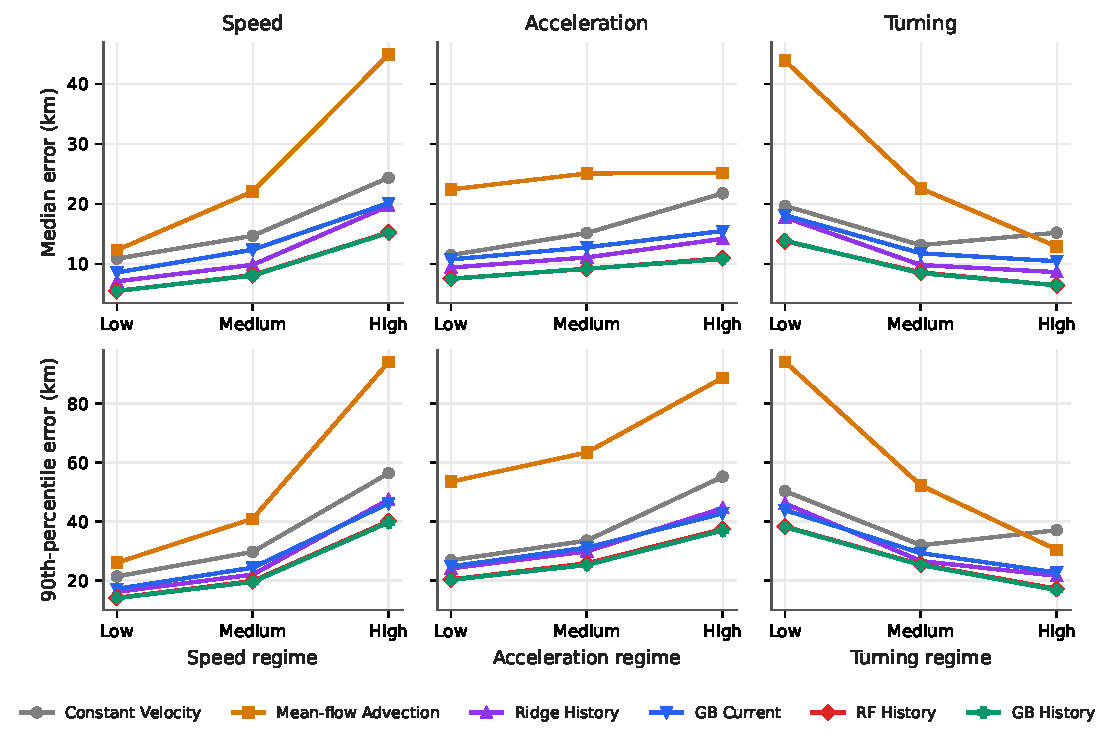
\includegraphics[width=\textwidth]{figures/generated/fig_motion_profiles.pdf}
  \caption{Median (top) and 90th-percentile (bottom) test error across speed, acceleration and turning regimes for six representative methods. Lines join regime summaries for readability only; the regimes are ordered categories. RF History and \GBH{} almost coincide. Re-plotted from \texttt{models/motion\_conditioned\_test\_errors.csv} (notebook cell 51).}
  \label{fig:motion}
\end{figure}

\paragraph{Speed.} Error rises steeply with recent speed for every method. For \GBH{} the median roughly triples from \SI{5.55}{km} (Low) to \SI{15.21}{km} (High), and P90 rises from \SI{14.0}{km} to \SI{39.7}{km} (bottom row of \cref{fig:motion}). The P90 profiles mirror the medians for every descriptor, so the patterns are not confined to typical forecasts. The relative advantage over CV shrinks with speed (49\% to 38\%), but the absolute advantage grows (\SIlist{5.4;6.6;9.2}{km}). Part of this gradient is geometric: a fixed directional error produces a larger position error the farther the drifter travels. Even the best model therefore remains least accurate, in absolute terms, for the fast drifters that move material farthest.

\paragraph{Acceleration.} Errors also increase with acceleration magnitude, but the pattern differs from speed. CV degrades fastest (median \SI{11.5}{}$\to$\SI{21.8}{km}), while \GBH{} degrades more slowly (\SI{7.5}{}$\to$\SI{10.8}{km}), so the relative gain rises from 34\% to 50\%. This is what one would expect if the history summaries capture changes in velocity that constant extrapolation ignores. The acceleration magnitude mixes changes in speed and direction, and for a given turning rate it scales with speed, so this descriptor is not independent of the other two.

\paragraph{Turning.} Contrary to the proposal's working hypothesis, which expected turning to be associated with \emph{larger} errors, errors are highest for the \emph{least} turning drifters (\GBH{} median \SI{13.91}{km}) and lowest for the most turning ones (\SI{6.48}{km}). Two further observations help interpret this. First, Mean-flow Advection, which is far worse than CV overall, beats CV in the High-turning regime (\SI{12.93}{} against \SI{15.23}{km}), and it is catastrophically wrong in the Low-turning regime (\SI{43.85}{km}). When a drifter is looping, its instantaneous velocity is a poor guide to its net 24-hour displacement. A climatology that predicts small net motion is then preferable, whereas in a straight, fast jet the climatology is far too slow. Second, the relative gain of \GBH{} over CV is largest under high turning (57.5\%), consistent with the history features summarising oscillatory or curved motion. These interpretations are plausible but untested. Because turning and speed are correlated, the turning pattern must be examined jointly with speed.

\subsection{Joint speed--turning analysis}
\Cref{fig:joint}a confirms a strong association between the two descriptors. Among Low-speed forecasts, 62.4\% are High-turning, whereas 71.8\% of High-speed forecasts are Low-turning, and the High-speed/High-turning cell contains only 3,816 forecasts (4.6\%) from 44 drifters. Much of the marginal ``high turning means low error'' pattern therefore reflects the fact that strongly turning drifters are usually slow.

\begin{figure}[!htbp]
  \centering
  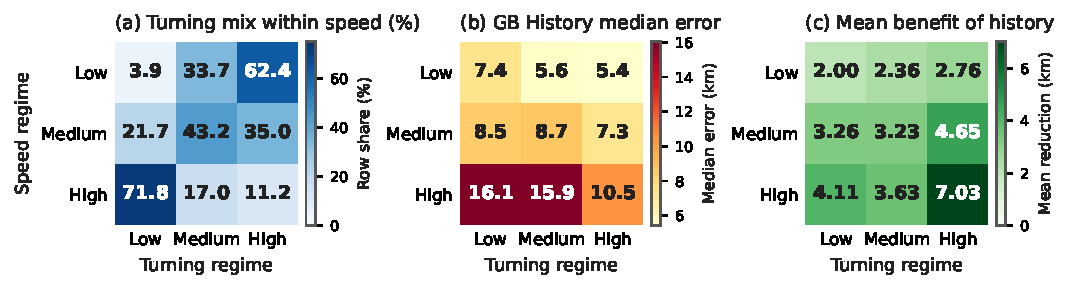
\includegraphics[width=\textwidth]{figures/generated/fig_joint_speed_turning.pdf}
  \caption{Joint speed--turning regimes on the test set (\num{82533} forecasts with defined turning). (a) Turning distribution within each speed regime (row \%). (b) Median \GBH{} error (km). (c) Mean paired benefit of history, $E^{\mathrm{GBC}}-E^{\mathrm{GBH}}$ (km); note that (b) shows medians and (c) shows means. Re-plotted from saved test predictions; values reproduce notebook cell 53.}
  \label{fig:joint}
\end{figure}

The association does not, however, explain the turning pattern away. Within each speed tertile, High-turning forecasts still have the lowest \GBH{} median error (\cref{fig:joint}b): \SI{16.06}{}, \SI{15.94}{} and \SI{10.47}{km} across turning regimes at High speed, and \SI{7.36}{}, \SI{5.57}{} and \SI{5.44}{km} at Low speed. The Medium-speed row is not monotone (\SI{8.48}{}, \SI{8.68}{}, \SI{7.26}{km}). The tertiles are broad, and the High-speed band includes every mean speed above \SI{0.40}{m\,s^{-1}}, so residual confounding by speed within a band cannot be excluded.

The mean benefit of history (\cref{fig:joint}c) increases with speed in every turning column and is largest in the High-turning column of every speed row. It ranges from \SI{2.00}{km} (Low speed, Low turning) to \SI{7.03}{km} (High speed, High turning). Part of the speed gradient is a scale effect, since larger errors leave more room for absolute improvement. The High-speed/High-turning cell is an exception to a pure scale explanation: its \GBH{} median error (\SI{10.5}{km}) is \emph{lower} than in the other High-speed cells, yet the benefit of history there is the largest.

\subsection{Uncertainty in the benefit of history}
\Cref{fig:boot}a gives drifter-cluster bootstrap intervals for the nine joint-regime benefits (\cref{tab:boot} in \cref{app:tables}). All nine point estimates are positive and every 95\% interval excludes zero. Even the smallest benefit, \SI{2.00}{km} (\SIrange{1.24}{2.71}{km}) for Low speed and Low turning, is distinguishable from zero after accounting for within-drifter dependence. The High-speed/High-turning interval is the widest (\SIrange{5.38}{9.17}{km}), reflecting its 44 contributing drifters.

\begin{figure}[!htbp]
  \centering
  \begin{subfigure}[t]{\textwidth}\centering
    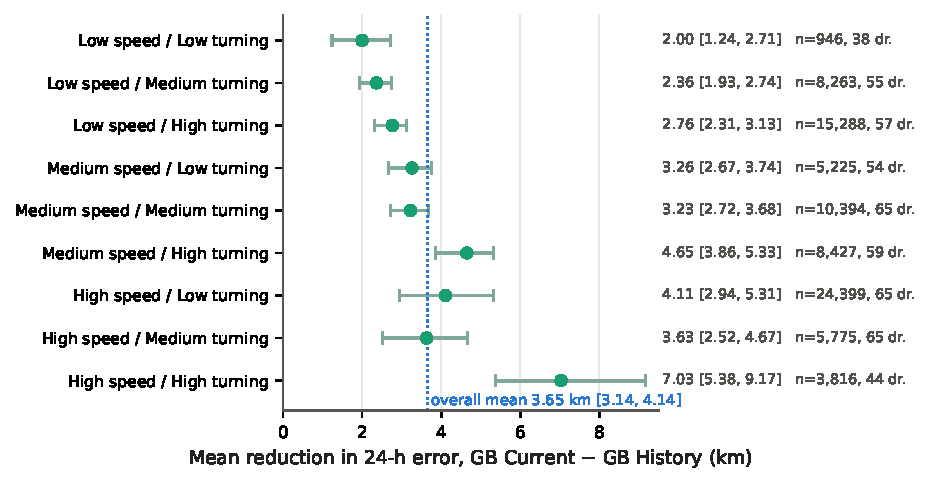
\includegraphics[width=0.92\linewidth]{figures/generated/fig_bootstrap_regimes.pdf}
    \caption{Mean benefit of history by joint regime, with 95\% intervals, cases and drifters}
  \end{subfigure}\\[3pt]
  \begin{subfigure}[t]{\textwidth}\centering
    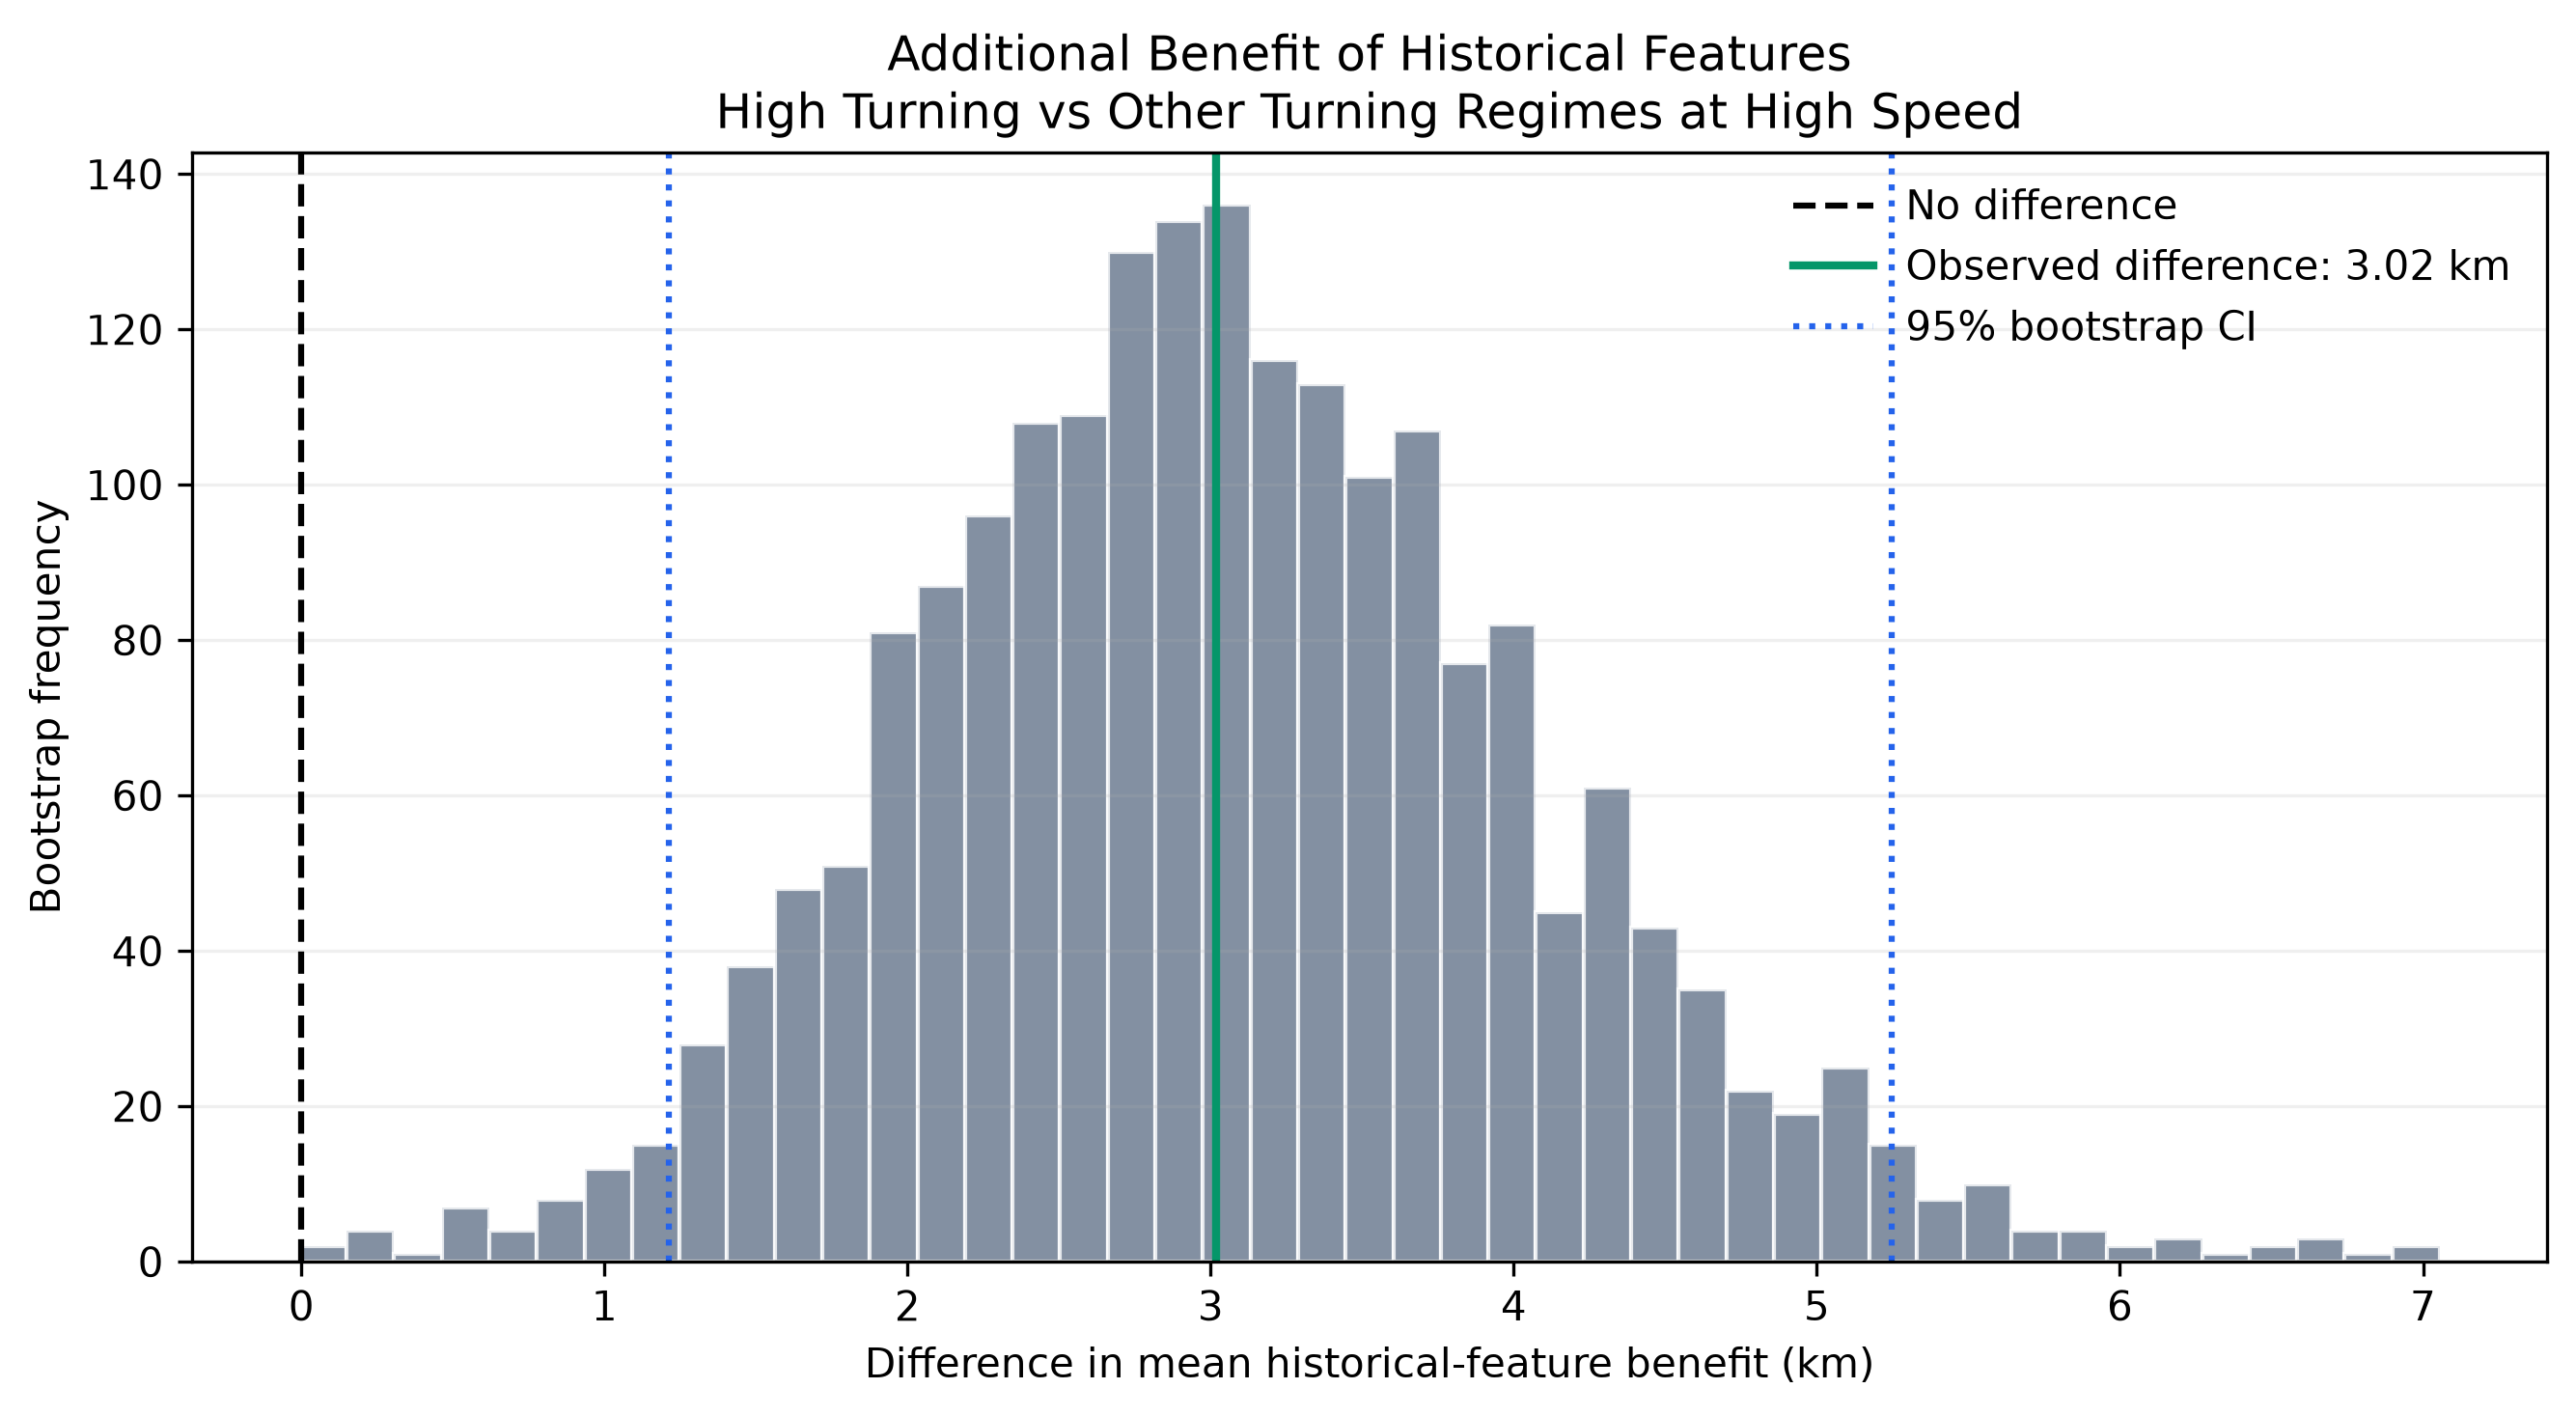
\includegraphics[width=0.62\linewidth]{figures/report_high_speed_turning_bootstrap_contrast.png}
    \caption{High-speed contrast: High vs Low/Medium turning}
  \end{subfigure}
  \caption{Drifter-cluster bootstrap (2,000 resamples of the 78 test drifters). (a) Mean paired benefit of history ($E^{\mathrm{GBC}}-E^{\mathrm{GBH}}$) with 95\% percentile intervals; the dotted line is the overall mean. Re-plotted from \texttt{models/history\_gain\_cluster\_bootstrap.csv} (cell 55). (b) Bootstrap distribution of the difference in mean benefit between High-turning and Low/Medium-turning forecasts within the High-speed regime (original figure, cell 57).}
  \label{fig:boot}
\end{figure}

Separate intervals for each regime do not by themselves test whether two regimes differ. We therefore estimated the contrast that motivated the analysis directly (\cref{fig:boot}b). Within the High-speed regime, the mean benefit was \SI{7.03}{km} for High-turning forecasts and \SI{4.02}{km} for Low/Medium-turning forecasts. The difference of \SI{3.02}{km} has a 95\% bootstrap interval of \SIrange{1.21}{5.25}{km}, which excludes zero. This contrast was defined \emph{after} inspecting \cref{fig:joint}c, it is one of many comparisons that could have been made, and no multiplicity adjustment was applied. It should therefore be read as strong exploratory evidence that history is especially valuable for fast drifters that are turning, to be confirmed on independent data, rather than as a pre-registered test. The analysis also does not separate turning from co-varying factors such as location or the eddy field.

\paragraph{Answer to the research question (motion).} In this dataset, 24-hour forecast difficulty is driven primarily by recent speed. Acceleration adds difficulty mainly for Constant Velocity. Turning is associated with \emph{lower} absolute error, largely through its negative association with speed. History improves forecasts in all regimes examined, and most clearly for fast, turning motion.
